\documentclass[11pt]{article} 
\usepackage[english]{babel}
\usepackage[utf8]{inputenc}
\usepackage[margin=0.5in]{geometry}
\usepackage{amsmath}
\usepackage{amsthm}
\usepackage{amsfonts}
\usepackage{amssymb}
\usepackage[usenames,dvipsnames]{xcolor}
\usepackage{graphicx}
\usepackage[siunitx]{circuitikz}
\usepackage{tikz}
\usepackage[colorinlistoftodos, color=orange!50]{todonotes}
\usepackage{hyperref}
\usepackage[numbers, square]{natbib}
\usepackage{fancybox}
\usepackage{epsfig}
\usepackage{soul}
\usepackage[framemethod=tikz]{mdframed}
\usetikzlibrary{positioning, automata, backgrounds}
\usepackage[shortlabels]{enumitem}
\usepackage[version=4]{mhchem}
\usepackage{multicol}
\usepackage{forest}
\usepackage{mathtools}
\usepackage{comment}
\usepackage{enumitem}
\usepackage[utf8]{inputenc}
\usepackage[linesnumbered,ruled,vlined]{algorithm2e}
\usepackage{listings}
\usepackage{color}
\usepackage[numbers]{natbib}
\usepackage{subfiles}
\usepackage{tkz-berge}


\newtheorem{prop}{Proposition}[section]
\newtheorem{thm}{Theorem}[section]
\newtheorem{lemma}{Lemma}[section]
\newtheorem{cor}{Corollary}[prop]

\theoremstyle{definition}
\newtheorem{definition}{Definition}

\theoremstyle{definition}
\newtheorem{required}{Problem}

\theoremstyle{definition}
\newtheorem{ex}{Example}

\newcommand{\interval}[4]{\draw (#2, #1) -- (#3, #1); % Usage: \interval{height}{start}{end}{label}
\draw (#2, #1-0.11) -- (#2, #1+0.11); % draw left whisker
\draw (#3, #1-0.11) -- (#3, #1+0.11); % draw right whisker
\node[] at (#2-0.25, #1) {#4};
}

\setlength{\marginparwidth}{3.4cm}
%#########################################################

%To use symbols for footnotes
\renewcommand*{\thefootnote}{\fnsymbol{footnote}}
%To change footnotes back to numbers uncomment the following line
%\renewcommand*{\thefootnote}{\arabic{footnote}}

% Enable this command to adjust line spacing for inline math equations.
% \everymath{\displaystyle}

% _______ _____ _______ _      ______ 
%|__   __|_   _|__   __| |    |  ____|
%   | |    | |    | |  | |    | |__   
%   | |    | |    | |  | |    |  __|  
%   | |   _| |_   | |  | |____| |____ 
%   |_|  |_____|  |_|  |______|______|
%%%%%%%%%%%%%%%%%%%%%%%%%%%%%%%%%%%%%%%

\title{
\normalfont \normalsize 
\textsc{CSCI 3104 Spring 2022 \\ 
Instructors: Profs. Chen and Layer} \\
[10pt] 
\rule{\linewidth}{0.5pt} \\[6pt] 
\huge Problem Set 2 \\
\rule{\linewidth}{2pt}  \\[10pt]
}
%\author{}
\date{}

\begin{document}

\definecolor {processblue}{cmyk}{0.96,0,0,0}
\definecolor{processred}{rgb}{200, 0, 0}
\definecolor{processgreen}{rgb}{0, 255, 0}
\DeclareGraphicsExtensions{.png}
\DeclareGraphicsExtensions{.gif}
\DeclareGraphicsExtensions{.jpg}

\maketitle


%%%%%%%%%%%%%%%%%%%%%%%%%
%%%%%%%%%%%%%%%%%%%%%%%%%%
%%%%%%%%%%FILL IN YOUR NAME%%%%%%%
%%%%%%%%%%AND STUDENT ID%%%%%%%%
%%%%%%%%%%%%%%%%%%%%%%%%%%
\noindent
Due Date \dotfill February 1, 2022 \\
Name \dotfill \textbf{Your Name} \\
Student ID \dotfill \textbf{Your Student ID} \\
Collaborators \dotfill \textbf{List Your Collaborators Here}

\tableofcontents

\section{Instructions}
 \begin{itemize}
	\item The solutions \textbf{should be typed}, using proper mathematical notation. We cannot accept hand-written solutions. \href{http://ece.uprm.edu/~caceros/latex/introduction.pdf}{Here's a short intro to \LaTeX.}
	\item You should submit your work through the \textbf{class Canvas page} only. Please submit one PDF file, compiled using this \LaTeX \ template.
	\item You may not need a full page for your solutions; pagebreaks are there to help Gradescope automatically find where each problem is. Even if you do not attempt every problem, please submit this document with no fewer pages than the blank template (or Gradescope has issues with it).

	\item You are welcome and encouraged to collaborate with your classmates, as well as consult outside resources. You must \textbf{cite your sources in this document.} \textbf{Copying from any source is an Honor Code violation. Furthermore, all submissions must be in your own words and reflect your understanding of the material.} If there is any confusion about this policy, it is your responsibility to clarify before the due date. 

	\item Posting to \textbf{any} service including, but not limited to Chegg, Reddit, StackExchange, etc., for help on an assignment is a violation of the Honor Code.

	\item You \textbf{must} virtually sign the Honor Code (see Section \ref{HonorCode}). Failure to do so will result in your assignment not being graded.
\end{itemize}


\section{Honor Code (Make Sure to Virtually Sign)} \label{HonorCode}

\begin{required}
\begin{itemize}
\item My submission is in my own words and reflects my understanding of the material.
\item Any collaborations and external sources have been clearly cited in this document.
\item I have not posted to external services including, but not limited to Chegg, Reddit, StackExchange, etc.
\item I have neither copied nor provided others solutions they can copy.
\end{itemize}

%\noindent In the specified region below, clearly indicate that you have upheld the Honor Code. Then type your name. 
\end{required}

\begin{proof}[Agreed (signature here).]
%% Typing "I agree to the above," followed by your name is sufficient.
\end{proof}


%%%%%%%%%%%%%%%%%%%%%%%%%%%%%%%%%%%%%%%%%%%%%%%%%%
\newpage
\section{Standard 5- BFS and DFS}
\subsection{Problem \ref{DFS1}}
\begin{required} \label{DFS1}
Consider a \textsf{Modified Connectivity} problem:
\begin{itemize}
\item \textsf{Instance:} Let $G(V, E)$ be a simple, undirected graph. Let $s, t \in V(G)$.
\item \textsf{Decision:} Given an integer $k\geq 1$,  is there a shortest path from $s$ to $t$ in $G$ that consists of $k$ edges? Here the length/weight of a path is defined as the number of edges of the path. 
\end{itemize}

\noindent \\ Do the following. [\textbf{Note:} There are parts (a) and (b). Part (b) is on the next page.]
\begin{enumerate}[label=(\alph*)]
\item Design an algorithm to solve the $\textsf{Modified Connectivity}$ problem. Your solution should provide enough detail that a CSCI 2270 student could reasonably be expected to implement your solution.
\begin{proof}[Answer for Part (a)]
%Your answer goes here
\end{proof}



\newpage
\item We say that the graph $G$ is \textit{connected} if for every pair of vertices $s, t \in V(G)$, there exists a path from $s$ to $t$. Design an algorithm to determine whether $G$ is connected. Your algorithm should only traverse the graph once - this means that you should \textbf{not} apply BFS or DFS more than once. Your solution should provide enough detail that a CSCI 2270 student could reasonably be expected to implement your solution.

\begin{proof}[Answer for Part (b)]
%Your answer goes here
\end{proof}
\end{enumerate}
\end{required}






\newpage
\subsection{Problem \ref{DFS2}} 
\begin{required} \label{DFS2}
Give an example of a simple, undirected, and unweighted graph $G(V, E)$ that has a single source shortest path tree which a \textbf{depth-first traversal} will not return for any ordering of its vertices. 
    Your answer must
    \begin{enumerate}[label=(\alph*)]
    	\item Provide a drawing of the graph $G$. [\textbf{Note:} We have provided TikZ code below if you wish to use \LaTeX \ to draw the graph. Alternatively, you may hand-draw $G$ and embed it as an image below, provided that (i) your drawing is legible and (ii) we do not have to rotate our screens to grade your work.]
    	\item Specify the single source shortest path tree $T = (V,E_T)$ by specifying $E_T$ and also specifying the root $s \in V$. [\textbf{Note:} You may again hand-draw this tree. If you wish, you may clearly mark the edges of $T$ on your drawing of $G$. Please make it easy on the graders to identify the edges of $T$.] 
    	\item Include a clear explanation of why the depth-first search algorithm we discussed in class will never produce $T$ for any orderings of the vertices.
    \end{enumerate}

\end{required}

\noindent 
\begin{proof}[Answer]
%Your proof goes here.
\end{proof}


\noindent The following provides a sample of how to draw graphs with \LaTeX. You may use the graph below, or you may come up with your own example.
\begin{center}
	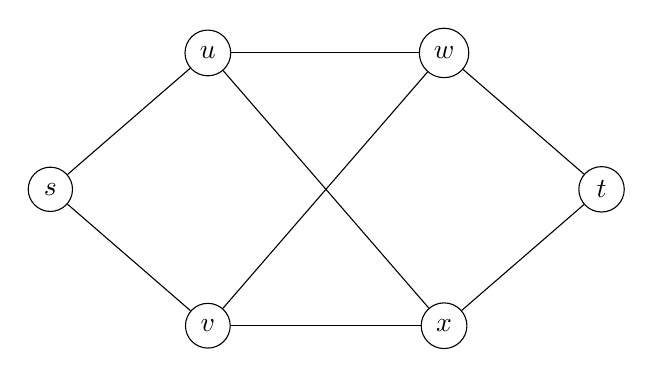
\begin{tikzpicture}[
		wide/.style={line width=4pt},
		every node/.style={circle,draw,minimum size=16},
		scale=2]
		\node (s) at (-0.5,0)            {$s$};
		\node (u) at ($ (0,0) + ( 60:1)$) {$u$};
		\node (v) at ($ (0,0) + (-60:1)$) {$v$};
		\node (w) at ($ (u) + ( 1.5,0 )$) {$w$};
		\node (x) at ($ (v) + ( 1.5,0 )$) {$x$};
		\node (t) at ($ (w) + (-60:1) + (0.5,0)$) {$t$};
		\draw (s) -- (u);
		\draw (u) -- (w);
		\draw (w) -- (t);

% Replace the line \draw (w) -- (t); with the line below (after deleting the % symbol to uncomment) in order to draw a thicker edge.
%		\draw[line width=3pt] (w) -- (t);


		\draw (s) -- (v);
		\draw (v) -- (x);
		\draw (x) -- (t);
		\draw (u) -- (x);    
		\draw (v) -- (w);
		
\end{tikzpicture}
\end{center}







\newpage
\subsection{Problem \ref{DFS4}}
\begin{required} \label{DFS4}
	Give an example of a simple, undirected, weighted graph such that a breadth-first traversal outputs a search-tree that is not a single source shortest path tree. (That is, BFS is not sufficiently powerful to solve the shortest-path problem on weighted graphs. This motivates Dijkstra's algorithm.) 
	Your answer must
	\begin{enumerate}[label=(\alph*)]
		\item Draw the graph $G = (V,E, w)$ by specifying $V$ and $E$, clearly labeling the edge weights.  [\textbf{Note:} We have provided TikZ code below if you wish to use \LaTeX \ to draw the graph. Alternatively, you may hand-draw $G$ and embed it as an image below, provided that (i) your drawing is legible and (ii) we do not have to rotate our screens to grade your work.]
		\item Specify a spanning tree $T(V, E_{T})$ that is returned by BFS, but is not a single-source shortest path tree. [\textbf{Note:} You may again hand-draw this tree. If you wish, you may clearly mark the edges of $T$ on your drawing of $G$. Please make it easy on the graders to identify the edges of $T$.] 

		\item Specify a valid single-source shortest path tree $T^{\prime} = (V,E_{T^{\prime}})$.  [\textbf{Note:} You may again hand-draw this tree. If you wish, you may clearly mark the edges of $T$ on your drawing of $G$. Please make it easy on the graders to identify the edges of $T$.] 

		\item Include a clear explanation of why the search-tree output by breadth-first search is not a valid single-source shortest path tree of $G$.
	\end{enumerate}
\end{required}


\begin{proof}[Answer]
%Your answer here.
\end{proof}

\noindent The following provides a sample of how to draw graphs with edge weights using \LaTeX. You may use the graph below, or you may come up with your own example.
\begin{center}
	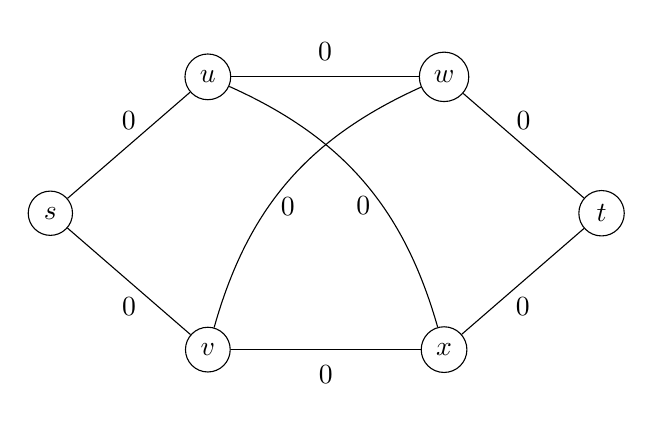
\begin{tikzpicture}[
		wide/.style={line width=4pt},
		every node/.style={circle,draw,minimum size=16},
		scale=2]
		\node (s) at (-0.5,0)            {$s$};
		\node (u) at ($ (0,0) + ( 60:1)$) {$u$};
		\node (v) at ($ (0,0) + (-60:1)$) {$v$};
		\node (w) at ($ (u) + ( 1.5,0 )$) {$w$};
		\node (x) at ($ (v) + ( 1.5,0 )$) {$x$};
		\node (t) at ($ (w) + (-60:1) + (0.5,0)$) {$t$};


% Replace the line \draw (w) -- (t); with the line below (after deleting the % symbol to uncomment) in order to draw a thicker edge.
%		\draw[line width=3pt] (w) -- (t);


		\draw (s) -- node[below, draw=none,fill=none]{0} (v);
		\draw (v) -- node[below, draw=none,fill=none]{0} (x);
		\draw (x) -- node[below, draw=none,fill=none]{0} (t);
		\draw (u) edge[bend left=25] node[below, draw=none,fill=none]{0} (x);    
		\draw (v) edge[bend left=25] node[below, draw=none,fill=none]{0} (w);
		\draw (s) -- node[above, draw=none,fill=none]{0} (u);
		\draw (u) -- node[above, draw=none,fill=none]{0} (w);
		\draw (w) -- node[above, draw=none,fill=none]{0} (t);		
\end{tikzpicture}
\end{center}
%%%%%%%%%%%%%%%%%%%%%%%%%%%%%%%%%%%%%%%%%%%%%%%%%%


\newpage
\section{Standard 6- Dijkstra's Algorithm}

\subsection{Problem \ref{Dijkstra0}}
\begin{required} \label{Dijkstra0}
Consider the weighted graph $G(V, E, w)$ pictured below. Work through Dijkstra's algorithm on the following graph, using the source vertex $E$. 
\begin{itemize}
\item Clearly include the contents of the priority queue, as well as the distance from $E$ to each vertex at each iteration.
\item If you use a table to store the distances, clearly label the keys according to the vertex names rather than numeric indices (i.e., \texttt{dist[`B']} is more descriptive than \texttt{dist[`1']}).
\item You do \textbf{not} need to draw the graph at each iteration, though you are welcome to do so. [This may be helpful scratch work, which you do not need to include.]
\end{itemize}


\begin{center}
\begin {tikzpicture}[-latex, auto, node distance =2 cm and 3cm, semithick]
\tikzstyle{blue}=[circle ,top color =white , bottom color = processblue!20 ,draw,processblue , text=blue , minimum width =1 cm];
\tikzstyle{red}=[circle ,top color =white , bottom color = processred!20 ,draw, processred , text=blue , minimum width =1 cm];
\tikzstyle{green}=[circle ,top color =white , bottom color = processgreen!20 ,draw, processgreen , text=blue , minimum width =1 cm];

	\node[blue] (A) {$A$};
	\node[blue] (C) [below right = of A] {$C$};
	\node[blue] (B) [below right = of C] {$B$};
	\node[blue] (E) [below left = of A] {$E$};
	\node[blue] (D) [below left = of E] {$D$};
	\node[blue] (H) [below right = of D] {$H$};
	\node[blue] (F) [right = of H] {$F$};

	\path (A) edge node[above] {$4$} (C);
	\path (E) edge node[left] {$9$} (A);

	\path (C) edge node[above] {$3$} (B);
	\path (B) edge node[below] {$6$} (F);

	\path (E) edge node[above] {$10$} (C);
	\path (C) edge node[above] {$2$} (F);

	\path (D) edge node[above] {$4$} (H);

	\path (E) edge node[above] {$20$} (F);
	\path (E) edge node[right] {$9$} (D);
	\end{tikzpicture}  
\end{center}

\end{required}

\begin{proof}[Answer]
%Your answer here
\end{proof}





\newpage
\subsection{Problem \ref{Dijkstra2}} 
\begin{required} \label{Dijkstra2}
You have three batteries, with capacities of 40, 25, and 16 Ah (Amp-hours), respectively. The 25 and 16-Ah batteries are fully charged (containing 25 Ah and 16 Ah, respectively), while the 40-Ah battery is empty, with 0 Ah. You have a battery transfer device which has a ``source'' battery position and a ``target'' battery position. When you place two batteries in the device, it instantaneously transfers as many Ah from the source battery to the target battery as possible. Thus, this device stops the transfer either when the source battery has no Ah remaining or when the destination battery is fully charged (whichever comes first).  \\

\noindent But battery transfers aren't free! The battery device is also hooked up to your phone by bluetooth, and automatically charges you a number of dollars equal to however many Ah it just transfered.  \\
	
\noindent The goal in this problem is to determine whether there exists a sequence of transfers that leaves exactly 10 Ah either in the 25-Ah battery or the 16-Ah battery, and if so, how little money you can spend to get this result. \\

\noindent Do the following.
\begin{enumerate}[label=(\alph*)]
\subsubsection{Problem 6\ref{Dijkstra2a}}
\item \label{Dijkstra2a} Rephrase this is as a graph problem. Give a precise definition of how to model this problem as a graph, and state the specific question about this graph that must be answered. [\textbf{Note:} While you are welcome to draw the graph, it is enough to provide 1-2 sentences clearly describing what the vertices are and when two vertices are adjacent. If the graph is weighted, clearly specify what the edge weights are.]

\begin{proof}[Answer]
%Your answer goes here.
\end{proof}

\newpage
\subsubsection{Problem 6\ref{Dijkstra2b}}
\item \label{Dijkstra2b} Clearly describe an algorithm to solve this problem. If you use an algorithm covered in class, it is enough to state that. If you modify an algorithm from class, clearly outline any modifications. Make sure to explicitly specify any parameters that need to be passed to the initial function call.

\begin{proof}[Answer]
%Your answer goes here
\end{proof}



\newpage
\subsubsection{Problem 6\ref{Dijkstra2c}}
\item \label{Dijkstra2c} Apply that algorithm to the question. Report and justify your answer. Here, justification includes the sequences of vertices visited and the total cost. 

\begin{proof}[Answer]
%Your answer goes here
\end{proof}

\end{enumerate}
\end{required}



\end{document} % NOTHING AFTER THIS LINE IS PART OF THE DOCUMENT



